\documentclass{beamer}
\usefonttheme{professionalfonts}% Now beamer didn't modify the math fonts
\usepackage{geometry}
\usepackage[]{tcolorbox}
\usepackage{varwidth}   %% provides varwidth environment
\usepackage{empheq}
\usepackage{adjustbox}


\newcommand*{\cajados}[1]{\noindent\fbox{%
\parbox{\textwidth}{%
    #1
}%
}}
\newcommand{\caja}[1]{\begin{empheq}[box=\fbox]{alignat*=8}
    #1
\end{empheq}}

\newcommand*{\objetivodos}[2]{#1 x_{1} + #2 x_{2}}
\newcommand*{\objetivotres}[3]{#1 x_{1} + #2 x_{2} + #3x_{3}}
\newcommand*{\restdos}[3]{#1 x_{1} + #2 x_{2} \le #3}
\newcommand*{\irestdos}[3]{#1 x_{1}  #2 x_{2} = #3}
\newcommand*{\iresttres}[4]{#1 x_{1}  #2 x_{2} #3x_{3} = #4}

\newcommand*{\resttres}[4]{#1 x_{1} + #2 x_{2} + #3 x_{3} \le #4}
\newcommand*{\restuno}[2]{#1 x_{1} \le #2}
\newcommand{\posit}[1]{x_{#1} \ge 0}

\newcommand{\R}{\mathbb{R}}
% \usepackage{tikz-cd}
\beamertemplatenavigationsymbolsempty
\setbeamertemplate{footline}[page number]{}
\setbeamerfont{footline}{size=\footnotesize}
\usepackage{tcolorbox}
\usepackage{biblatex}
% \usepackage{tikzcd}
\usetheme{Copenhagen}



\title[]{Clase tutorial 02: Programación lineal pt.1.}
% \subtitle{Workshop de LOREL 2024.}
\date{14 de Agosto de 2024.}
\author[]{ Investigación operativa.
  }
\institute{Universidad de San Andrés}
% \titlegraphic{\hfill\includegraphics[height=1.5cm]{logo.pdf}}

\begin{document}
\maketitle

\begin{frame}[fragile]{Programación lineal.}
  \tcajita{¿Qué es la programación lineal (PL)?}{Es un método para conseguir el resultado óptimo (sea máxima
  ganancia o menor costo) en un modelo matemático en el cual
  tanto los restricciones como el objetivo resultan ser \textbf{lineales}.}
  
\end{frame}

\begin{frame}[fragile]{Problema de PL general.}
  En general un problema de PL tiene los siguientes componentes.
  \begin{align*} \LARGE  
    Z  & \quad \quad \text{función objetivo} \\ 
    x_{j}  & \quad \quad \text{variable de decisión} \\
    c_{j}  & \quad \quad \text{aumento del objetivo $Z$ al aumentar en una unidad} \\
    & \quad \quad \text{la variable de decisión $x_{j}$} \\
    b_{i}  & \quad \quad \text{cantidad de recurso $i$ disponible} \\
    a_{ij}  & \quad \quad \text{cantidad de recurso $i$} \\
    & \quad \quad \text{consumido por cada unidad de la actividad $j$}
  \end{align*}
\end{frame}

\begin{frame}[fragile]{Ejemplo.}
  \tcajita{Ejemplo.}{
    Resolver el siguiente problema de programación lineal.
    \begin{align*}
        \max \ \objetivodos{3}{} \\
        \restdos{2}{}{25} \\ 
        \restdos{}{3}{15} \\ 
        \posit{1} \\ 
        \posit{2}
    \end{align*}
  }
  \pause 
  \alert{¿Cuáles son la función objetivo, las variables de decisión y los parámetros del problema?}
\end{frame}

\begin{frame}[fragile]{Ejemplo de problema pt.1.}
\footnotesize
Una empresa (Wyndor Glass Co.) produce puertas y ventanas. Deciden poner en producción dos productos nuevos:
\begin{itemize}
  \item \textbf{Producto 1}: Una ventana de 2m de altura con marco de aluminio.
  \item \textbf{Producto 2}: Una ventana colgante de 3m con marco de madera.
\end{itemize}


Wyndor tiene 3 fábricas que cumplen funciones diferentes. El producto 1 requiere producción de la fábrica 1 y 3 mientras que el producto 2 requiere de las plantas 2 y 3. La división de marketing de la empresa hizo un estudio en el cual llegaron a la conclusión de que podrían vender la misma cantidad de ambos productos. 

Sin embargo, como ambos están compitiendo por tiempo de producción en la fábrica 3 (el cuál es limitado), la compañía debe decidir cuánto hacer de cada uno para obtener el mayor retorno posible. 

Queremos saber cuánto de cada producto debemos fabricar para \textbf{maximizar el retorno teniendo en cuenta las horas de producción limitadas de las fábricas.}
\end{frame}

\begin{frame}[fragile]{Ejemplo de problema pt.2.}
  La compañía fabrica por lotes por lo tanto nuestras variables de decisión las vamos a tomar como el número de lotes por semana.
  \bigskip
  \footnotesize

  \begin{tabular}{||p{0.15\linewidth} | p{0.15\linewidth} | 
    p{0.15\linewidth}| p{0.2\linewidth}||}
    \hline
    & \multicolumn{2}{|c|}{ Horas necesarias de producción por lote.} & \\
    \hline
    Planta &Producto 1 &Producto 2 & Tiempo disponible por semana de producción.\\
    \hline
    1   & 1    & 0 &  4  \\
    2   & 0    & 2 &  12 \\
    3   & 3    & 2 &  18 \\
    \hline
    Ganancia por lote & \$3000 & \$5000 &  \\
    \hline
  \end{tabular}
\end{frame}

\begin{frame}[fragile]{Ejemplo de problema pt.3.}
  \begin{center}
      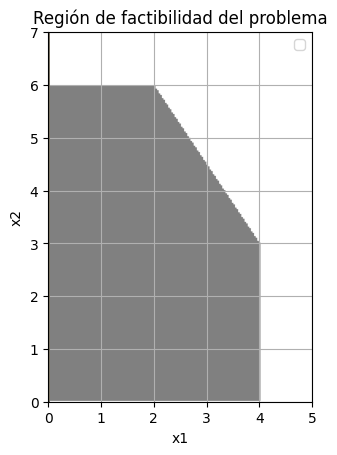
\includegraphics[scale=0.68]{01-factibilidad.png}
  \end{center}
\end{frame}

\begin{frame}[fragile]{Ejemplo de problema pt.4.}
  Matemáticamente podemos representar el problema de la siguiente manera.

  \tcajita{Problema.}{
    \begin{align*}
        \max \ Z  &= 3000x_{1} + 5000x_{2} \\
        \\
        x_{1} &\le 4 \\
        2x_{2} &\le 12 \\
        3x_{1} + 2x_{2} &\le 18 \\
        x_{1} &\ge 0 \\
        x_{2} &\ge 0
    \end{align*}
  }
\end{frame}
\begin{frame}[fragile]{Traducción del problema a python.}
  Abrimos colab y para traducir este problema a PICOS.
\end{frame}


\begin{frame}[fragile]{Representación matricial de los problemas de PL.}
  Si denotamos 
  \begin{align*}
    x &= (x_{1}, \dots, x_{n}) \\
    c &= (c_{1}, \dots, c_{n}) \\
    b &= (b_{1}, \dots, b_{m}) \\
  \end{align*}
  y la matriz 
  \[
  a = \begin{bmatrix}
    a_{11} & a_{12} &\dots &a_{1n} \\
    a_{21} & a_{22} &\dots &a_{2n} \\
    \vdots & \vdots & \ddots &\vdots \\
    a_{m1} & a_{m2} &\dots &a_{mn} \\
  \end{bmatrix}
  \]

  Entonces el problema se puede escribir como 
  \caja{\min Z = cx^{t} \ \text{sujeta a} \ \  ax^{t} \le b}
\end{frame}

\begin{frame}[fragile]{Traducción del problema a python (versión matricial)}
  Abrimos colab (nuevamente) para traducir este problema a PICOS.
\end{frame}

\begin{frame}[fragile]{Problema para pensar}
  \tcajita{Problema}{Una empresa tiene sólo tres empleados (Diego, Ludmila y Bruno) que hacen dos tipos de
  ventanales a mano: con marco de madera y con marco de aluminio. 
  \newline
  La ganancia es de \$180
  por cada ventanal con marco de madera y de \$90 por cada uno con marco de aluminio.
  Diego hace marcos de madera y puede terminar 6 al día. Ludmila hace 4 marcos de aluminio
  por día. Bruno forma y corta el vidrio y puede hacer 48 metros cuadrados de vidrio por día. 
  \newline
  Cada ventanal con marco de madera emplea 6 metros cuadrados de vidrio y cada uno de aluminio 8
  metros cuadrados. 
  \newline
  \textbf{¿Cuántos ventanales de cada tipo debe producir al día para maximizar la
  ganancia total?}}
\end{frame}

\end{document}
